
\chapter{El primer rayo de Sol -- II}
\label{sec:el-primer-rayo-de-sol-ii}

\lettrine[ante=\raisebox{-1.5ex}{\Large ---},lines=2]{N}{os quedó}
pendiente extrudir el polígono ---An\-to\-nia empezó el capítulo yendo
directamente al grano.

    \begin{center}
    \begin{lstlisting}
alto_pixel = 2;
ancho_pixel = 6;
radio_semicilindro = 30;
H = radio_semicilindro+10;

module rayo_de_sol(alfa){
  D=H/tan(alfa);
  vertices=[[-alto_pixel/2,0],
            [D-alto_pixel/2,H],
            [D+alto_pixel/2,H],
            [alto_pixel/2,0]];
  linear_extrude(ancho_pixel)
    polygon(vertices);
}
 
rayo_de_sol(alfa=60);
    \end{lstlisting}
  \end{center}

  \begin{figure}[t]
    \centering
  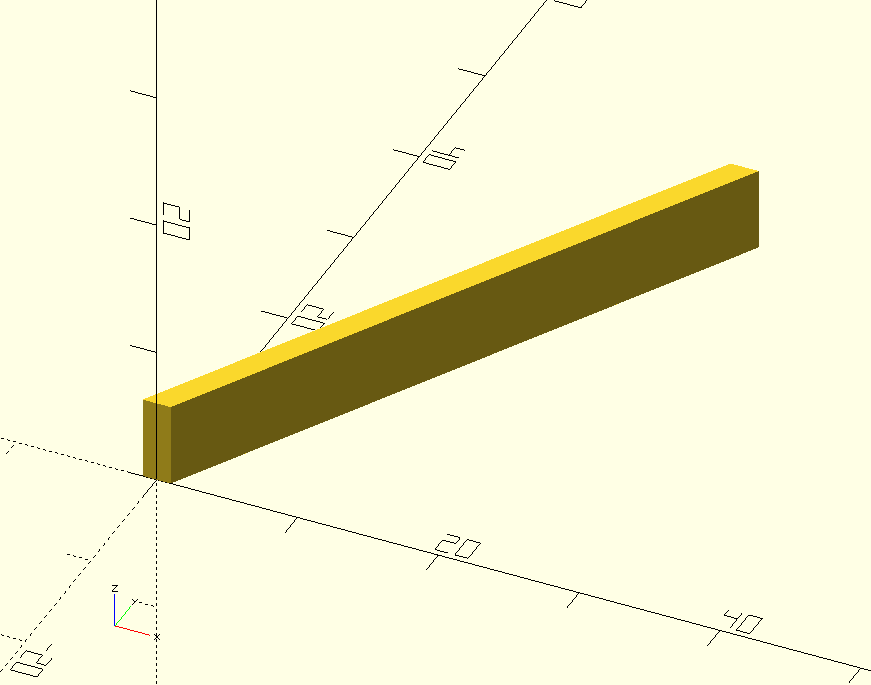
\includegraphics[width=.6\textwidth]{imagenes/rayo-extrudido-1}  
  \caption{Rayo de Sol extrudido en espera de ser rotado.}
    \label{fig:rayo-extrudido-1}
  \end{figure}
  
  

  ---Y ahora, ¡a rotarlo! ---intervino Cecilia, riendo y tomando el
  teclado para sí.

%    \begin{center}
    \begin{lstlisting}
alto_pixel = 2;
ancho_pixel = 6;
radio_semicilindro = 30;
H = radio_semicilindro+10;

module rayo_de_sol(alfa){
  D=H/tan(alfa);
  vertices=[[-alto_pixel/2,0],
            [D-alto_pixel/2,H],
            [D+alto_pixel/2,H],
            [alto_pixel/2,0]];
  rotate([90,0,0])
    linear_extrude(ancho_pixel)
      polygon(vertices);
}
 
rayo_de_sol(alfa=60);
    \end{lstlisting}
 % \end{center}

  \begin{figure}[t]
    \centering
  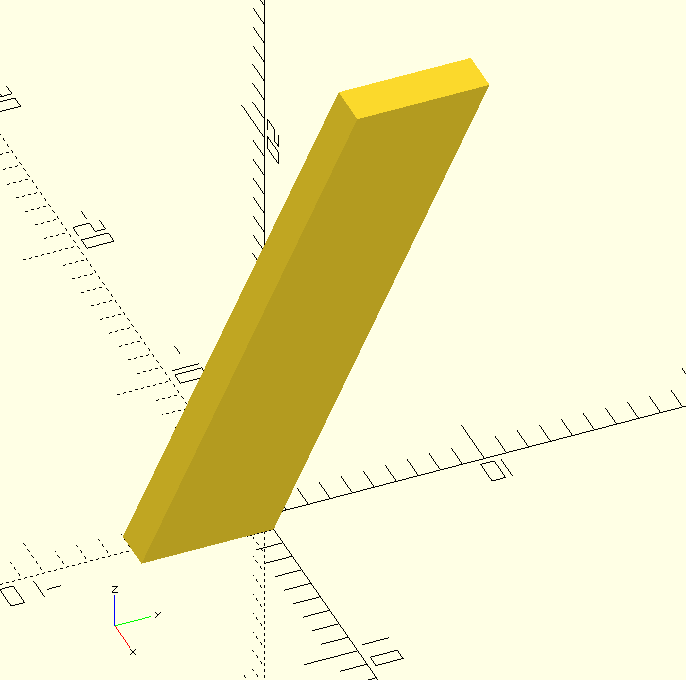
\includegraphics[width=.48\textwidth]{imagenes/rayo-extrudido-2}    
    \caption{Primer rayo de Sol rotado por Cecilia.}
    \label{fig:rayo-extrudido-2}
  \end{figure}

  

  Cecilia admiró feliz el resultado en la figura
  \ref{fig:rayo-extrudido-2}: estaban cada vez más cerca de su ansiado
  reloj de Sol digital. Sin embargo, un detalle congeló su sonrisa:
  advirtió que la base del rayo no estaba centrada en el origen, sino
  un poco corrida:

  ---Antonia, el rayo nos quedó del lado de las \coord{Y} negativas:
  ¿no será un problema? ¿Te parece que lo traslademos en
  \texttt{ancho\_pixel/2} a lo largo de ese eje?

  Antonia sonrió, enarcando las cejas con admiración:

  ---Bien por notar el problema, y mejor por encontrar una
  solución. En realidad, no sé si será un problema más adelante; en
  todo caso, siempre conviene que los módulos se comporten de la
  manera más simple posible. En este caso, todo parece indicar que lo
  más natural es que la base del rayo de Sol esté centrada ---Antonia
  hizo una pausa, y su mirada parecía ver más allá del monitor---.
  Efectivamente, puede resolverse con una mera traslación; basta
  intercalar la indicación \lstinline!translate([0,ancho_pixel/2,0])!
  entre las líneas 11 y 12 de tu texto. Pero hay otra forma:


    \begin{lstlisting}
alto_pixel = 2;
ancho_pixel = 6;
radio_semicilindro = 30;
H = radio_semicilindro+10;

module rayo_de_sol(alfa){
  D=H/tan(alfa);
  vertices=[[-alto_pixel/2,0],
            [D-alto_pixel/2,H],
            [D+alto_pixel/2,H],
            [alto_pixel/2,0]];
  linear_extrude(ancho_pixel,center=true)
    polygon(vertices);
}
 
rayo_de_sol(alfa=60);
\end{lstlisting}

\begin{figure}[ht]
  \centering
  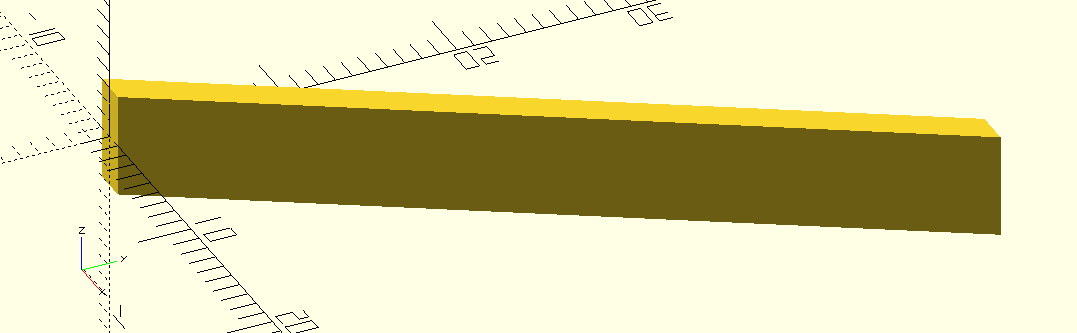
\includegraphics[width=.8\textwidth]{imagenes/rayo-extrudido-3}  
  \caption{Antonia extruye el polígono del rayo de Sol con la opción
    \lstinline!center=true!.}
  \label{fig:rayo-extrudido-3}
\end{figure}


\guillemotright Cuando agregás la prescripción \lstinline!center=true!
a la transformación \lstinline!linear_extrude! (como hice en la línea
12), la extrusión se realiza centrada con respecto al plano
\coord{XY}. Ahora sí, si lo rotamos:



    \begin{lstlisting}
alto_pixel = 2;
ancho_pixel = 6;
radio_semicilindro = 30;
H = radio_semicilindro+10;

module rayo_de_sol(alfa){
  D=H/tan(alfa);
  vertices=[[-alto_pixel/2,0],
            [D-alto_pixel/2,H],
            [D+alto_pixel/2,H],
            [alto_pixel/2,0]];
  rotate([90,0,0])
    linear_extrude(ancho_pixel,center=true)
      polygon(vertices);
}
 
rayo_de_sol(alfa=60);
\end{lstlisting}


\begin{figure}[ht]
  \centering
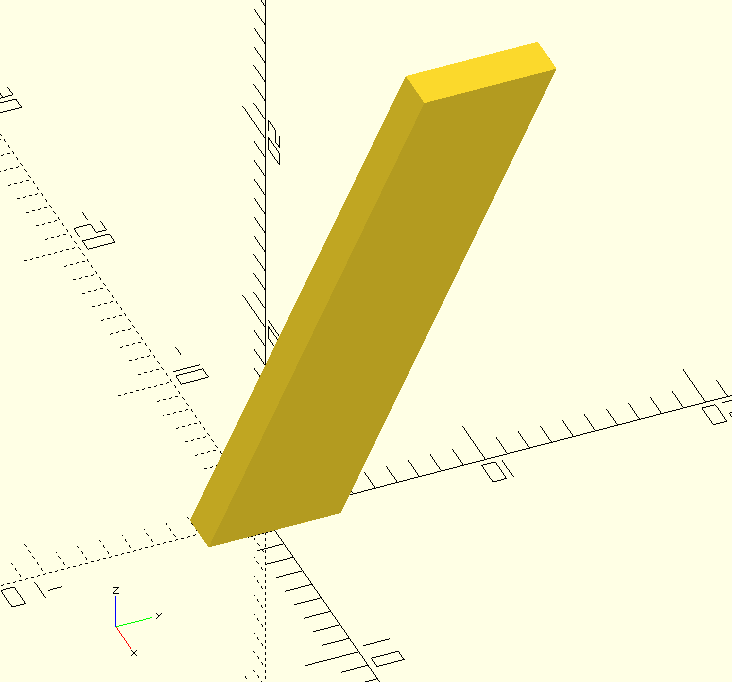
\includegraphics[width=.5\textwidth]{imagenes/rayo-extrudido-4}  
  \caption{Rayo de Sol correctamente centrado.}
  \label{fig:rayo-extrudido-4}
\end{figure}



Cecilia aplaudió con indisimulada alegría la figura
\ref{fig:rayo-extrudido-4}. Antonia seguía concentrada con la mirada
en dirección al monitor:

---Te confieso que no estoy segura de cuál de las dos soluciones sea
la mejor. Deberíamos tener en cuenta que nuestro reloj estará
atravesado por multitud de rayos, todos los cuales deberán ser
calculados por la computadora: siempre es bueno, en esos `cuellos de
botella' computacionales, elegir el algoritmo más eficiente ---Antonia
suspiró---. No conozco cómo funciona internamente el motor de
\openscad{}; supongo que lo mejor que podemos hacer es probar ambas
soluciones, y medir cuánto tarda cada una. Es un buen momento para
colocar un comentario al respecto:




\begin{lstlisting}
module rayo_de_sol(alfa){
  D=H/tan(alfa);
  vertices=[[-alto_pixel/2,0],
            [D-alto_pixel/2,H],
            [D+alto_pixel/2,H],
            [alto_pixel/2,0]];
// TODO: medir la duracion de esta solucion
//       y la de esta otra:
// translate([0,ancho_pixel/2,0])
//       Ojo: borrar 'center=true' abajo
  rotate([90,0,0])
   linear_extrude(ancho_pixel,center=true)
    polygon(vertices);
}
\end{lstlisting}


Cecilia estaba demasiado feliz como para detenerse en esos detalles;
además, otra idea súbitamente se impuso a su atención.

\section{¿Un rayo de Sol alternativo?}

---¡Antonia! ¡Pará! ---exclamó Cecilia, con tono vi\-bran\-te---.  Dejame
probar... A ver... ¿No se puede hacer un rayo de Sol así..? ---y tomó
el teclado con decisión, mientras daba forma a su incipiente idea
escribiéndola.

\begin{lstlisting}
module otro_rayo_de_sol(alfa) {
  rotate([-(90-alfa),0,0])
   translate([-ancho_pixel/2,-alto_pixel/2,0])
    cube([ancho_pixel,alto_pixel,H]);  
}

otro_rayo_de_sol(alfa=60);
\end{lstlisting}


\begin{figure}[ht]
  \centering
  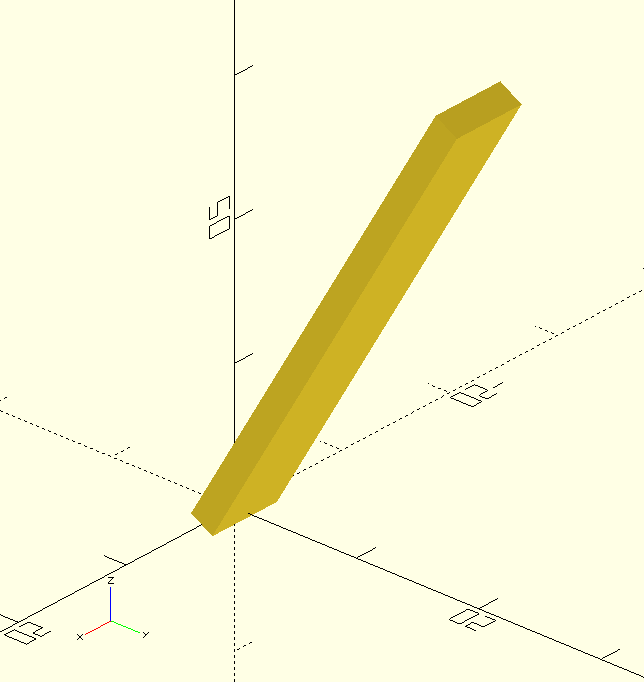
\includegraphics[width=.5\textwidth]{imagenes/otro-rayo}
  \caption[Rayo de Sol alternativo]{Un rayo de Sol alternativo,
    propuesto por Cecilia con entusiasmo.}
  \label{fig:otro-rayo}
\end{figure}
  
Cecilia se mostraba decididamente radiante mientras contemplaba la
figura \ref{fig:otro-rayo}. <<¿Para qué usar un polígono>> \mbox{---pen}\-só---
<<si podemos usar un elemental cubo?>>. Esperó una felicitación de
Antonia, o al menos un comentario, pero en vano: cuando volteó para
mirarla, encontró en ella sólo un gesto de displicente reserva.

---Yo también caí en esa trampa al principio ---confesó
An\-to\-\mbox{nia---.} La idea de un cubo se nos presenta eficaz,
incluso elegante; pero un detalle nefasto me demostró toda su
perversidad.\footnote{¡Eh..! ¿Será para tanto? (Nota del
  Editor)}$^,$\footnote{No: me agarró un ataque de retórica,
  nomás. (Nota de Antonia)}$^,$\footnote{Ah, listo; todo bien. (Nota
  del Editor)} Dejame que te muestre... ---Antonia se puso a escribir,
frente la atenta mirada de su amiga.

\begin{figure}[h]
  \centering
    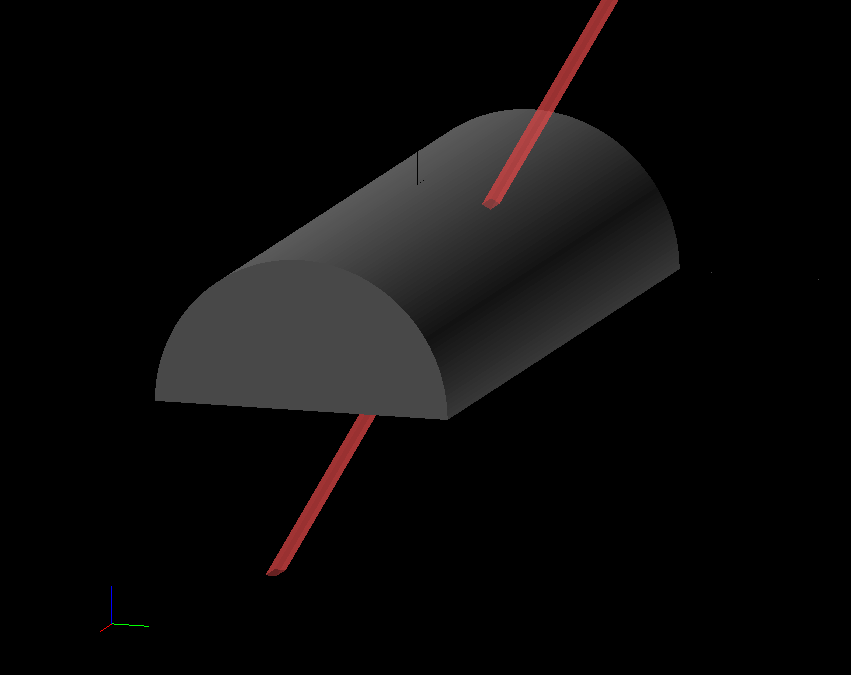
\includegraphics[width=.55\textwidth]{imagenes/otro-rayo-60}
    \caption[Rayo de Sol alternativo II]{Primer ejemplo con el que
      Antonia trata de disuadir a Cecilia de emplear su rayo de Sol
      alternativo.}
\label{fig:otro-rayo-60}
\end{figure}
  

\guillemotright En la figura \ref{fig:otro-rayo-60} te agregué un piso
para que vieras la marca que tu rayo de Sol, una vez atravesado el
reloj, dejaría en el mismo. ¿No notás nada raro? ---preguntó Antonia.

Cecilia respondió encogiéndose de hombros y enarcando las cejas.

---Sí, entiendo ---dijo Antonia---; no es tan evidente aún. A ver si
lo miramos bien de costado ---agregó, produciendo la figura
\ref{fig:otro-rayo-60-perfil}.

\begin{figure}[ht]
  \centering
    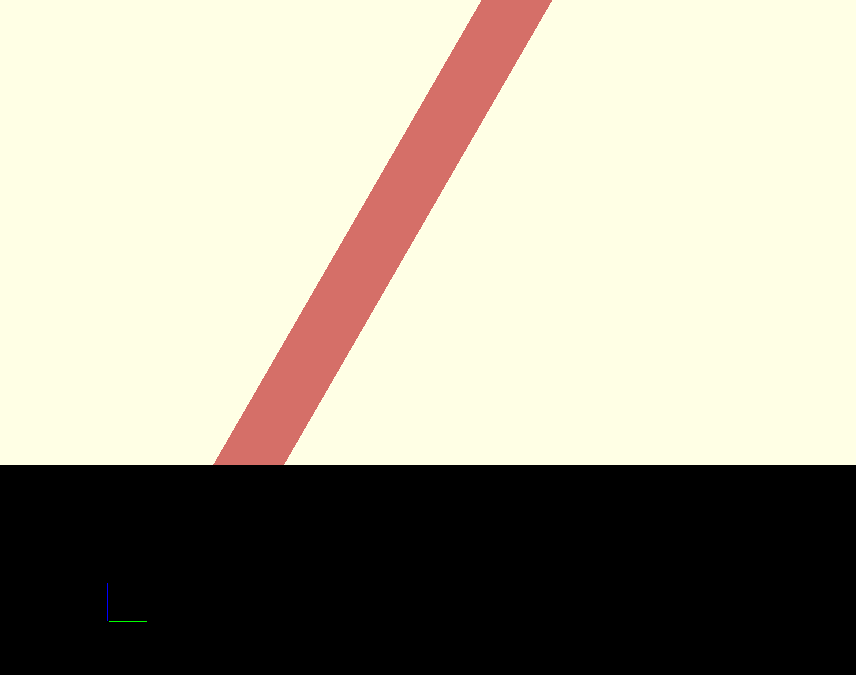
\includegraphics[width=.5\textwidth]{imagenes/otro-rayo-60-perfil}
    \caption[Rayo de Sol alternativo III]{Antonia sigue tratando de
      disuadir a Cecilia de emplear su rayo de Sol alternativo.}
    \label{fig:otro-rayo-60-perfil}
  \end{figure}


  ---Hmmm... tampoco ---confesó Cecilia.

  ---¿Y con un ángulo más bajo..? ---intentó Antonia ahora con la
  figura \ref{fig:otro-rayo-30}.


  \begin{figure}[ht]
  \centering
    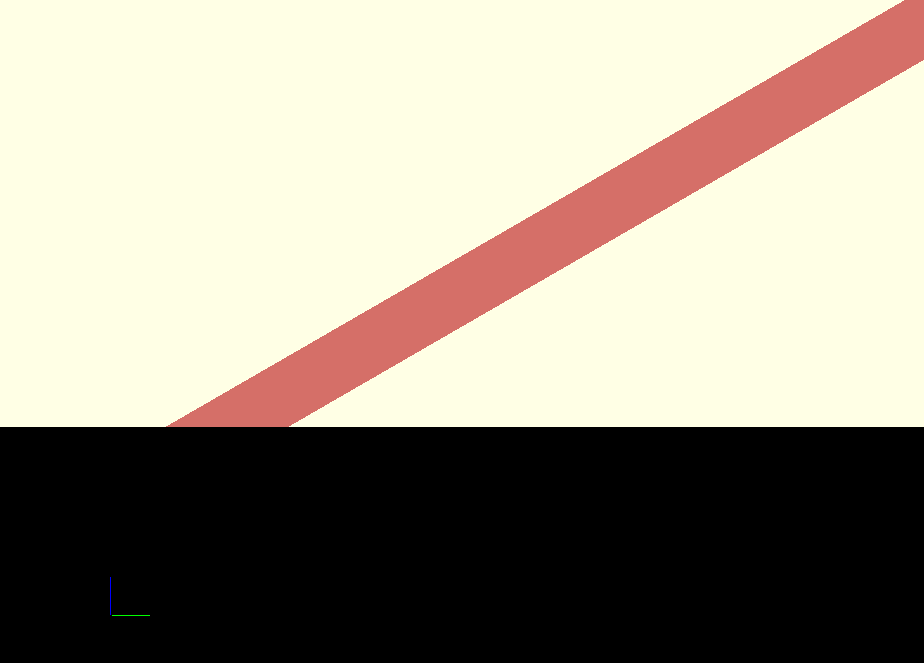
\includegraphics[width=.5\textwidth]{imagenes/otro-rayo-30}
    \caption[Rayo de Sol alternativo IV]{Antonia no ceja en su intento
      de disuadir a Cecilia de emplear su rayo de Sol alternativo.}
\label{fig:otro-rayo-30}
\end{figure}



    \begin{figure}[h!]
  \centering
    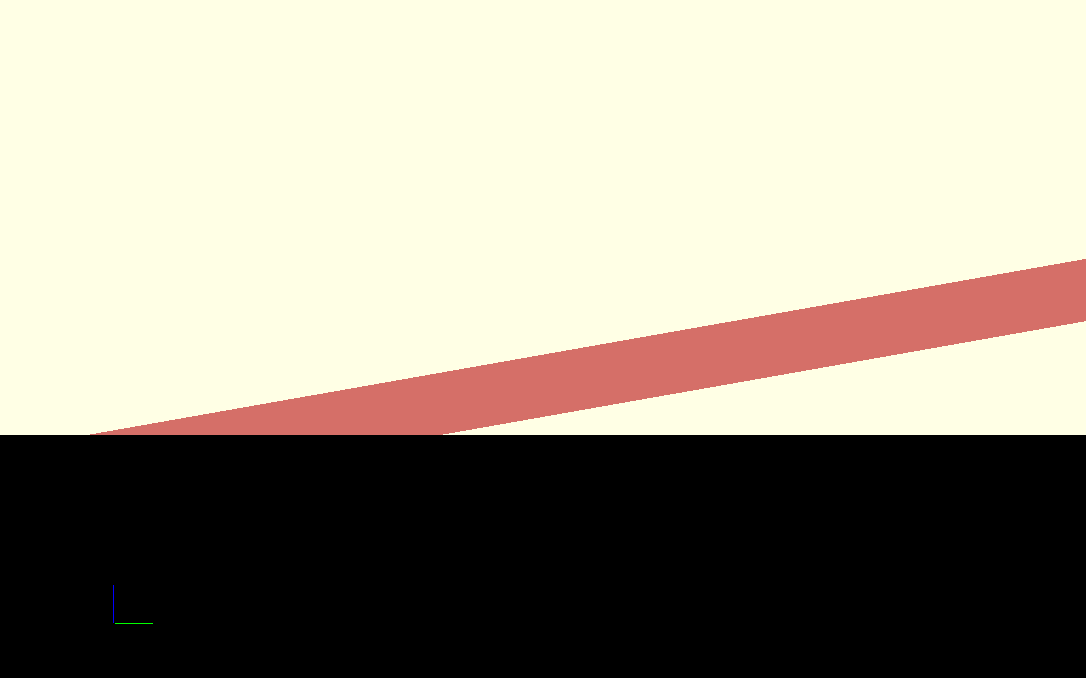
\includegraphics[width=.5\textwidth]{imagenes/otro-rayo-10}
    \caption[Rayo de Sol alternativo V]{Último intento de Antonia para
      disuadir a Cecilia de emplear su rayo de Sol alternativo.}%\vspace{128in}
\label{fig:otro-rayo-10}
\end{figure}

A Cecilia le pareció empezar a comprender.

---¿Y con 10$^{\circ}$..? ---Antonia suplicó señalando la figura
\ref{fig:otro-rayo-10}.  

---¡Claro! ---Cecilia se golpeó suavemente la frente con una
mano---. ¡La mancha de luz en el piso comienza a alargarse!  Lo que
debe medir \texttt{alto\_pixel} es la intersección del rayo con la
horizontal, no su sección transversal; por eso dibujaste el polígono
como lo hiciste.

---Por eso dibujé el polígono así \emph{al final} ---Antonia subrayó
estas últimas palabras---. Al principio lo hice como vos. Ésa es una
de las razones por las que me gusta escribir: aclara mis ideas.

Cecilia y Antonia se miraron, sonriendo.

  

%%% Local Variables:
%%% mode: latex
%%% TeX-master: "../libro"
%%% End:
